\section{Results}
\label{sec:results}

Figure \ref{fig:dynamics} shows the initial sea surface height (solid black) and compares the adjusted height and velocity profiles between numerical (solid) and analytical (dashed) solutions. Overall, there is good agreement in shape and magnitude. There are small discrepancies close to the boundaries where the numerical solution underestimates sea surface height and meridional velocity.
	\begin{figure}[htbp]
		\centering
		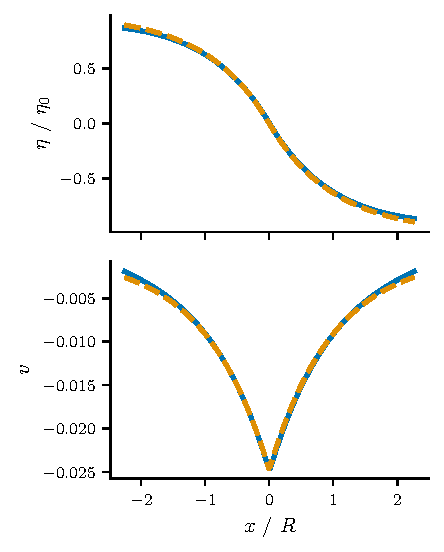
\includegraphics{dynamics_comparison}
		\caption{Upper: relative sea surface height. Lower: meridional velocity. Solid line shows numerical result, while dashed line shows analytical results. Parameters: $D_0=4000\,\text{m}$, $f_0=10^{-4}\,\text{m} / \text{s}^2$}
		\label{fig:dynamics}
	\end{figure}

The time evolution of relative potential (blue) and kinetic energy (orange) of the system is shown in Figure \ref{fig:energetics}. The black lines marks a 1/3 and 2/3. We see that $V$ and $K$ fluctuate initially before converging to 2/3 for the potential energy and 1/3 for the kinetic energy, in agreement with theory.
	\begin{figure}[htbp]
		\centering
		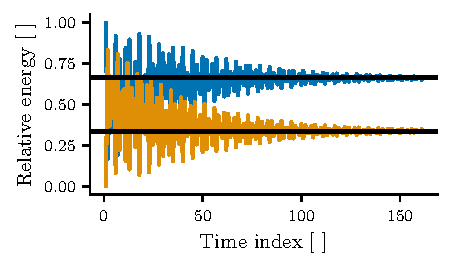
\includegraphics{energetics}
		\caption{Relative energies where blue line shows potential energy and orange line shows kinetic energy. The horizontal black lines marks a 1/3 and 2/3. Parameters: $D_0=4000\,\text{m}$, $f_0=10^{-4}\,\text{m} / \text{s}^2$}
		\label{fig:energetics}
	\end{figure}

The effect of depth is illustrated in Figure \ref{fig:energetics_d} where the upper plot shows a shallow basin and the lower plot a deep basin. In the shallow basin, the fraction of potential energy has increased compared with Figure \ref{fig:energetics}, while the opposite is true for the kinetic energy. Additionally, the fluctuations remain around the same, larger, magnitude throughout the entire integration period. In the deep basin, the opposite case is true where the potential energy fraction has decreased and the energy converges to a value faster with smaller fluctuations compared with Figure \ref{fig:energetics}.
	\begin{figure}[htbp]
		\centering
		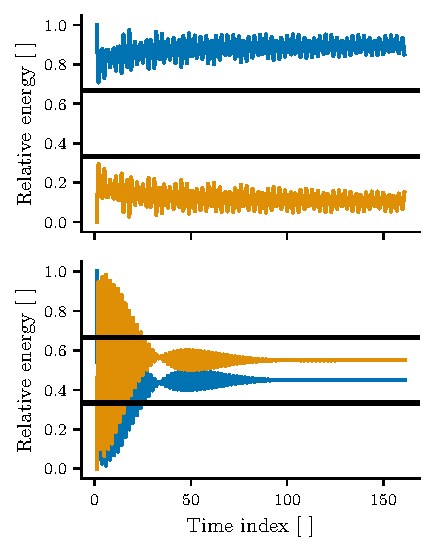
\includegraphics{energetics_d}
		\caption{Relative energies where blue line shows potential energy and orange line shows kinetic energy for $D_0 = 500 \,\text{m}$ (upper) and $D_0 = 10000\,\text{m}$ (lower). The horizontal black lines marks a 1/3 and 2/3. Here $f_0=10^{-4}\,\text{m} / \text{s}^2$}
		\label{fig:energetics_d}
	\end{figure}

Figure \ref{fig:energetics_f} shows the results of a smaller and larger planetary vorticity relative to $f_0 = 10^4\, \text{m} / \text{s}^2$. A lower planetary vorticity decreases the potential energy fraction and yields faster convergence, while the opposite is the case when increasing the planetary vorticity.
	\begin{figure}[htbp]
		\centering
		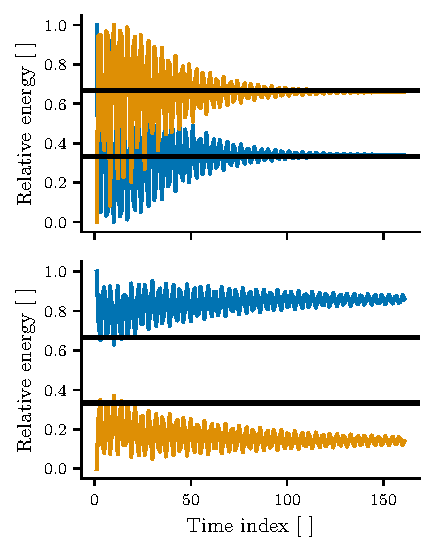
\includegraphics{energetics_f}
		\caption{Relative energies where blue line shows potential energy and orange line shows kinetic energy for $f_0=0.5 \cdot 10^{-4}\,\text{m} / \text{s}^2$ (upper) and $f_0=2 \cdot 10^{-4}\, \text{m} / \text{s}^2$ (lower). The horizontal black lines marks a 1/3 and 2/3. Here $D_0 = 4000\, \text{m}$.}
		\label{fig:energetics_f}
	\end{figure}